\documentclass[aspectratio=169, xcolor=dvipsnames]{beamer}

% --- Theme Setup ---
\usetheme{Madrid}
\usecolortheme{default}

% --- Packages ---
\usepackage{graphicx}
\usepackage{xcolor}
\usepackage{booktabs}
\usepackage{hyperref}
\usepackage{adjustbox}
\usepackage{amssymb}
\usepackage{amsmath}
\usepackage{listings}
\usepackage{caption}
\usepackage{tikz}

\lstset{
  basicstyle=\ttfamily\small,
  keywordstyle=\color{blue}\bfseries,
  stringstyle=\color{red},
  showstringspaces=false,
  breaklines=true
}

% --- Title Information ---
\title{Module 20}
\subtitle{Entity-Relationship Model/3}
\author{Milav Dabgar}
\institute{www.milav.in}
\date{\today}

\begin{document}

% Title Slide
\begin{frame}
    \titlepage
\end{frame}

\begin{frame}{Module Recap}
    \begin{itemize}[<+->]
        \item ER Diagram for ER Models
        \item Translation of ER Models to Relational Schema
    \end{itemize}
\end{frame}

\begin{frame}{Module Objectives}
    \begin{block}{Goals}
        \begin{itemize}[<+->]
            \item To understand extended features of ER Model
            \item To discuss various design issues
        \end{itemize}
    \end{block}
\end{frame}

\begin{frame}{Module Outline}
    \begin{itemize}[<+->]
        \item Extended ER Features
        \item Design Issues
    \end{itemize}
\end{frame}

\section{ER Features}
\begin{frame}
  \vfill
  \centering
  \begin{beamercolorbox}[sep=8pt,center,shadow=true,rounded=true]{title}
    \usebeamerfont{title}Extended ER Features\par%
  \end{beamercolorbox}
  \vfill
\end{frame}

\begin{frame}{Non-binary Relationship Sets}
    \begin{itemize}[<+->]
        \item Most relationship sets are binary
        \item There are occasions when it is more convenient to represent relationships as non-binary
        \item ER Diagram with a Ternary Relationship
    \end{itemize}
    \begin{center}
        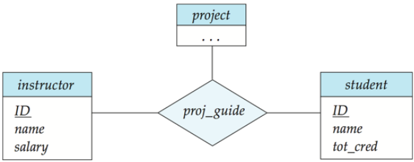
\includegraphics[width=0.6\textwidth]{../Lecture 4.5_artifacts/image_000006_9908d4c99df43cd94a3ae4699639456460d3f5f2ca4908536276ee15bdbf4a17.png}
    \end{center}
\end{frame}

\begin{frame}{Cardinality Constraints on Ternary Relationship}
    \begin{itemize}[<+->]
        \item We allow at most one arrow out of a ternary (or greater degree) relationship to indicate a cardinality constraint
        \item For example, an arrow from \texttt{proj\_guide} to \texttt{instructor} indicates each student has at most one guide for a project
        \item If there is more than one arrow, there are two ways of defining the meaning.
        \item For example, a ternary relationship $R$ between $A$, $B$ and $C$ with arrows to $B$ and $C$ could mean
        \begin{itemize}
            \item[$\triangleright$] a) Each $A$ entity is associated with a unique entity from $B$ and $C$ or
            \item[$\triangleright$] b) Each pair of entities from $(A, B)$ is associated with a unique $C$ entity, and each pair $(A, C)$ is associated with a unique $B$
        \end{itemize}
        \item Each alternative has been used in different formalisms
        \item To avoid confusion we outlaw more than one arrow
    \end{itemize}
\end{frame}

\begin{frame}{Specialization: ISA}
    \begin{block}{Definition}
        \begin{itemize}[<+->]
            \item \textbf{Top-down design process}: We designate sub-groupings within an entity set that are distinctive from other entities in the set
            \item These sub-groupings become lower-level entity sets that have attributes or participate in relationships that do not apply to the higher-level entity set
            \item Depicted by a triangle component labeled ISA (e.g., instructor 'is a' person)
            \item \textbf{Attribute inheritance}: A lower-level entity set inherits all the attributes and relationship participation of the higher-level entity set to which it is linked
        \end{itemize}
    \end{block}
\end{frame}

\begin{frame}{Specialization: ISA (2)}
    \begin{itemize}[<+->]
        \item Overlapping: employee and student
        \item Disjoint: instructor and secretary
        \item Total and Partial
    \end{itemize}
    \begin{center}
        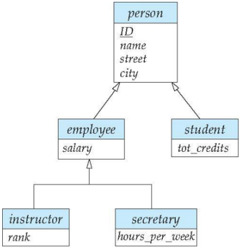
\includegraphics[width=0.45\textwidth]{../Lecture 4.5_artifacts/image_000010_b2c74e5d6a04040572182b98912b6a9c5f5e9964bf4a96f15c3d9d2cadd33501.png}
    \end{center}
\end{frame}

\begin{frame}{Representing Specialization via Schema}
    \begin{itemize}[<+->]
        \item \textbf{Method 1:}
        \begin{itemize}
            \item[$\triangleright$] Form a schema for the higher-level entity
            \item[$\triangleright$] Form a schema for each lower-level entity set, include primary key of higher-level entity set and local attributes
        \end{itemize}
        \item \textbf{Drawback}: Getting information about, an employee requires accessing two relations, the one corresponding to the low-level schema and the one corresponding to the high-level schema
    \end{itemize}
    
    \begin{table}[]
        \centering
        \begin{tabular}{|l|l|}
        \hline
        \textbf{schema} & \textbf{attributes} \\ \hline
        person & ID, name, street, city \\ 
        student & ID, tot\_cred \\ 
        employee & ID, salary \\ \hline
        \end{tabular}
    \end{table}
\end{frame}

\begin{frame}{Representing Specialization as Schema (2)}
    \begin{itemize}[<+->]
        \item \textbf{Method 2:}
        \begin{itemize}
            \item[$\triangleright$] Form a schema for each entity set with all local and inherited attributes
        \end{itemize}
        \item \textbf{Drawback}: name, street and city may be stored redundantly for people who are both students and employees
    \end{itemize}
    
    \begin{table}[]
        \centering
        \begin{tabular}{|l|l|}
        \hline
        \textbf{schema} & \textbf{attributes} \\ \hline
        person & ID, name, street, city \\ 
        student & ID, name, street, city, tot\_cred \\ 
        employee & ID, name, street, city, salary \\ \hline
        \end{tabular}
    \end{table}
\end{frame}

\begin{frame}{Generalization}
    \begin{block}{Definition}
        \begin{itemize}[<+->]
            \item \textbf{Bottom-up design process}: Combine a number of entity sets that share the same features into a higher-level entity set
            \item Specialization and generalization are simple inversions of each other; they are represented in an ER diagram in the same way
            \item The terms specialization and generalization are used interchangeably
        \end{itemize}
    \end{block}
\end{frame}

\begin{frame}{Design Constraints on a Specialization / Generalization}
    \begin{itemize}[<+->]
        \item \textbf{Completeness constraint}: Specifies whether or not an entity in the higher-level entity set must belong to at least one of the lower-level entity sets within a generalization
        \begin{itemize}
            \item[$\triangleright$] \textbf{total}: an entity must belong to one of the lower-level entity sets
            \item[$\triangleright$] \textbf{partial}: an entity need not belong to one of the lower-level entity sets
        \end{itemize}
        \item Partial generalization is the default. We can specify total generalization in an ER diagram by adding the keyword total in the diagram and drawing a dashed line from the keyword to the corresponding hollow arrow-head to which it applies (for a total generalization), or to the set of hollow arrow-heads to which it applies (for an overlapping generalization).
        \item The \texttt{student} generalization is total. All student entities must be either graduate or undergraduate. Because the higher-level entity set arrived at through generalization is generally composed of only those entities in the lower-level entity sets, the completeness constraint for a generalized higher-level entity set is usually total.
    \end{itemize}
    \begin{center}
        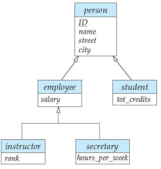
\includegraphics[width=0.6\textwidth]{../Lecture 4.5_artifacts/image_000016_9704c53a6842eeb22f40c6f422f7faacf259de4e5a17999300a7a19310ba2f91.png}
    \end{center}
\end{frame}

\begin{frame}{Aggregation}
    \begin{itemize}[<+->]
        \item Consider the ternary relationship \texttt{proj\_guide}, which we saw earlier
        \item Suppose we want to record evaluations of a student by a guide on a project
    \end{itemize}
    \begin{center}
        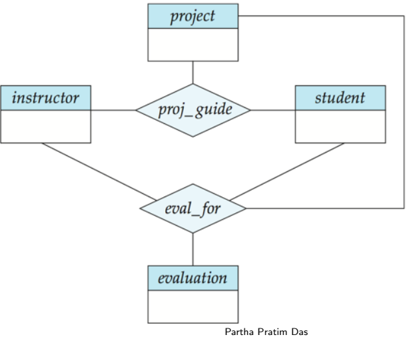
\includegraphics[width=0.6\textwidth]{../Lecture 4.5_artifacts/image_000018_f7a9fb800c801f952a17a08da3b1f7bb0509a5db64e6f1a8d9af4832937caaac.png}
    \end{center}
\end{frame}

\begin{frame}{Aggregation (2)}
    \begin{itemize}[<+->]
        \item Relationship sets \texttt{eval\_for} and \texttt{proj\_guide} represent overlapping information
        \begin{itemize}
            \item[$\triangleright$] Every \texttt{eval\_for} relationship corresponds to a \texttt{proj\_guide} relationship
            \item[$\triangleright$] However, some \texttt{proj\_guide} relationships may not correspond to any \texttt{eval\_for} relationships
            \item[$\triangleright$] $\triangleright$ So we cannot discard the \texttt{proj\_guide} relationship
        \end{itemize}
        \item Eliminate this redundancy via aggregation
        \begin{itemize}
            \item[$\triangleright$] Treat relationship as an abstract entity
            \item[$\triangleright$] Allows relationships between relationships
            \item[$\triangleright$] Abstraction of relationship into new entity
        \end{itemize}
    \end{itemize}
\end{frame}

\begin{frame}{Aggregation (3)}
    \begin{itemize}[<+->]
        \item Eliminate this redundancy via aggregation without introducing redundancy, the following diagram represents:
        \item A student is guided by a particular instructor on a particular project
        \item A student, instructor, project combination may have an associated evaluation
    \end{itemize}
    \begin{center}
        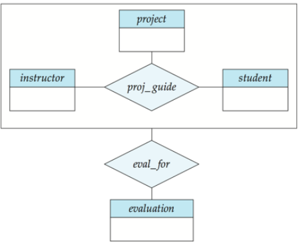
\includegraphics[width=0.6\textwidth]{../Lecture 4.5_artifacts/image_000021_840c0a62a336334fc76dbc061e7598296261d71fb3f9edcaae450a966963cc81.png}
    \end{center}
\end{frame}

\begin{frame}{Representing Aggregation via Schema}
    \begin{itemize}[<+->]
        \item To represent aggregation, create a schema containing
        \begin{itemize}
            \item[$\triangleright$] Primary key of the aggregated relationship,
            \item[$\triangleright$] The primary key of the associated entity set
            \item[$\triangleright$] Any descriptive attributes
        \end{itemize}
        \item In our example:
        \begin{itemize}
            \item[$\triangleright$] The schema \texttt{eval\_for} is: \texttt{eval\_for (s\_ID, project\_id, i\_ID, evaluation\_id)}
            \item[$\triangleright$] The schema \texttt{proj\_guide} is redundant
        \end{itemize}
    \end{itemize}
\end{frame}

\section{Design Issues}
\begin{frame}
  \vfill
  \centering
  \begin{beamercolorbox}[sep=8pt,center,shadow=true,rounded=true]{title}
    \usebeamerfont{title}Design Issues\par%
  \end{beamercolorbox}
  \vfill
\end{frame}

\begin{frame}{Entities vs. Attributes}
    \begin{itemize}[<+->]
        \item Use of entity sets vs. attributes
        \item Use of phone as an entity allows extra information about phone numbers (plus multiple phone numbers)
    \end{itemize}
    \begin{center}
        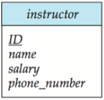
\includegraphics[width=0.45\textwidth]{../Lecture 4.5_artifacts/image_000025_358bea9acb6e77ac7d2e283fcd8422d971c6fad59593a2605599af81ee4c61d9.png}
        \hfill
        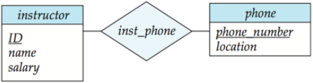
\includegraphics[width=0.45\textwidth]{../Lecture 4.5_artifacts/image_000026_b1c12ac38ef4562bfd926cb905fde75d0fdbbba28a196b1a17a8c4317a5be3a3.png}
    \end{center}
\end{frame}

\begin{frame}{Entities vs Relationship Sets}
    \begin{itemize}[<+->]
        \item Use of entity sets vs. relationship sets
        \begin{itemize}
            \item[$\triangleright$] Possible guideline is to designate a relationship set to describe an action that occurs between entities
        \end{itemize}
    \end{itemize}
    \begin{center}
        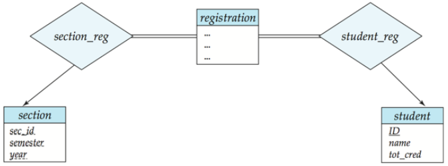
\includegraphics[width=0.6\textwidth]{../Lecture 4.5_artifacts/image_000028_019547ff0d45a72072cb4df9f055426f05799405b64120771ff6f8fbc7a21c17.png}
    \end{center}
    \begin{itemize}[<+->]
        \item Placement of relationship attributes
        \begin{itemize}
            \item[$\triangleright$] For example, attribute \texttt{date} as attribute of \texttt{advisor} or as attribute of \texttt{student}
        \end{itemize}
    \end{itemize}
\end{frame}

\begin{frame}{Binary vs Non-Binary Relationships}
    \begin{itemize}[<+->]
        \item Although it is possible to replace any non-binary (n-ary, for $n > 2$) relationship set by a number of distinct binary relationship sets, a n-ary relationship set shows more clearly that several entities participate in a single relationship
        \item Some relationships that appear to be non-binary may be better represented using binary relationships
        \begin{itemize}
            \item[$\triangleright$] For example, a ternary relationship \texttt{parents}, relating a child to his/her father and mother, is best replaced by two binary relationships, \texttt{father} and \texttt{mother}
            \item[$\triangleright$] Using two binary relationships allows partial information (e.g., only mother being known)
        \end{itemize}
        \item But there are some relationships that are naturally non-binary
        \begin{itemize}
            \item[$\triangleright$] Example: \texttt{proj\_guide}
        \end{itemize}
    \end{itemize}
\end{frame}

\begin{frame}{Binary vs Non-Binary Relationships (2): Conversion}
    \begin{itemize}[<+->]
        \item In general, any non-binary relationship can be represented using binary relationships by creating an artificial entity set.
        \item Replace $R$ between entity sets $A$, $B$ and $C$ by an entity set $E$, and three relationship sets:
        \begin{enumerate}
            \item $R_A$, relating $E$ and $A$
            \item $R_B$, relating $E$ and $B$
            \item $R_C$, relating $E$ and $C$
        \end{enumerate}
        \item Create an identifying attribute for $E$ and add any attributes of $R$ to $E$
        \item For each relationship $(a_i, b_i, c_i)$ in $R$, create
        \begin{itemize}
            \item[$\triangleright$] a) a new entity $e_i$ in the entity set $E$
            \item[$\triangleright$] b) add $(e_i, a_i)$ to $R_A$
            \item[$\triangleright$] c) add $(e_i, b_i)$ to $R_B$
            \item[$\triangleright$] d) add $(e_i, c_i)$ to $R_C$
        \end{itemize}
    \end{itemize}
\end{frame}

\begin{frame}{Binary vs Non-Binary Relationships (3): Conversion}
    \begin{itemize}[<+->]
        \item Also need to translate constraints
        \item Translating all constraints may not be possible
        \item There may be instances in the translated schema that cannot correspond to any instance of R.
        \begin{itemize}
            \item[$\triangleright$] Exercise: add constraints to the relationships $R_A$, $R_B$ and $R_C$ to ensure that a newly created entity corresponds to exactly one entity in each of entity sets $A$, $B$ and $C$
        \end{itemize}
        \item We can avoid creating an identifying attribute by making $E$, a weak entity set (described shortly) identified by the three relationship sets
    \end{itemize}
\end{frame}

\begin{frame}{ER Design Decisions}
    \begin{itemize}[<+->]
        \item The use of an attribute or entity set to represent an object
        \item Whether a real-world concept is best expressed by an entity set or a relationship set
        \item The use of a ternary relationship versus a pair of binary relationships
        \item The use of a strong or weak entity set
        \item The use of specialization/generalization - contributes to modularity in the design
        \item The use of aggregation - can treat the aggregate entity set as a single unit without concern for the details of its internal structure
    \end{itemize}
\end{frame}

\begin{frame}{Symbols Used in ER Notation}
    \begin{center}
        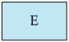
\includegraphics[width=0.9\textwidth,height=0.15\textheight,keepaspectratio]{../Lecture 4.5_artifacts/image_000036_1afb4260bb3a23d766a316f4c0987056adc2b68f32cb11527e79dc6bc688acf7.png}
    \end{center}
    \begin{center}
        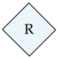
\includegraphics[width=0.9\textwidth,height=0.15\textheight,keepaspectratio]{../Lecture 4.5_artifacts/image_000037_fc38f640a1cca8f4ef2b81b6c2e0c531ffd682721fda7f458c9fbdad5f944c3a.png}
    \end{center}
    \begin{center}
        
\includegraphics[width=0.9\textwidth,height=0.15\textheight,keepaspectratio]{../Lecture 4.5_artifacts/image_000038_98efc726f14f6ccba012f08af46993b103c129c4d624b37afa803d90d2f6b8c3.png}
    \end{center}
    \begin{center}
        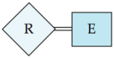
\includegraphics[width=0.9\textwidth,height=0.15\textheight,keepaspectratio]{../Lecture 4.5_artifacts/image_000039_bde2f54d4f5f4bd3440033251766c166e76f2450bd9a67da6c78facbef6f64ab.png}
    \end{center}
\end{frame}

\begin{frame}{Symbols Used in ER Notation (Cont.)}
    \begin{center}
        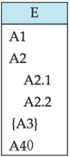
\includegraphics[width=0.9\textwidth,height=0.2\textheight,keepaspectratio]{../Lecture 4.5_artifacts/image_000040_cd784027eb2f560ff4570f0f74336a092ef072b3708362e691bd66c9fae533ea.png}
    \end{center}
    \begin{center}
        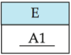
\includegraphics[width=0.9\textwidth,height=0.2\textheight,keepaspectratio]{../Lecture 4.5_artifacts/image_000041_583678cbaa156532988c8e16376b14426668f0d6f2ea4db96477793dd66b950c.png}
    \end{center}
    \begin{center}
        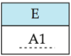
\includegraphics[width=0.9\textwidth,height=0.2\textheight,keepaspectratio]{../Lecture 4.5_artifacts/image_000042_0f03d88f453bfe6506983299defcc3ecf8f7471ba6f53ebf780f4f760732395f.png}
    \end{center}
\end{frame}

\begin{frame}{Symbols Used in ER Notation (2)}
    \begin{center}
        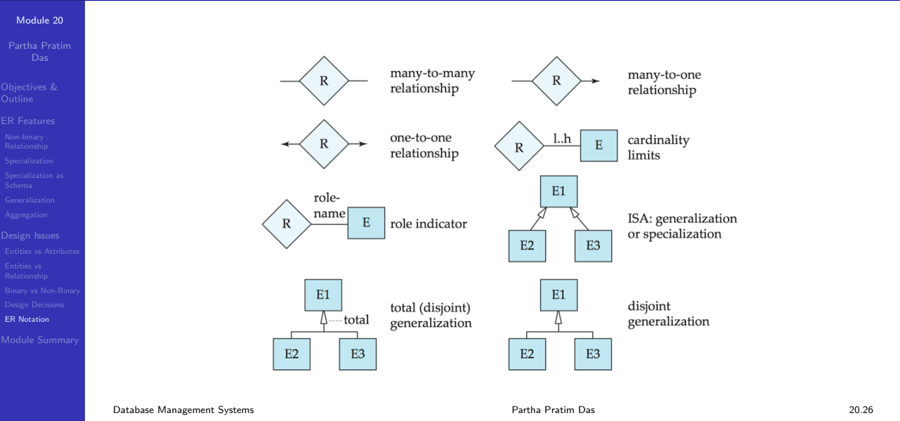
\includegraphics[width=0.9\textwidth]{../Lecture 4.5_artifacts/image_000044_eb0994f299837f25a41b795168657ba78dcb7abbfeba24acda9223959949ca35.png}
    \end{center}
\end{frame}

\begin{frame}{Symbols Used in ER Notation (3): Alternate}
    \begin{itemize}[<+->]
        \item Chen, IDE1FX, . . .
    \end{itemize}
    \begin{center}
        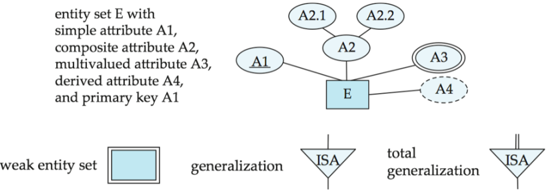
\includegraphics[height=0.7\textheight]{../Lecture 4.5_artifacts/image_000046_d491ed6bde473a164f099a4a086d46c4b6900f34a9bcc2f3d6fae8406197fc1a.png}
    \end{center}
\end{frame}

\begin{frame}{Symbols Used in ER Notation (4): Alternates}
    \begin{center}
        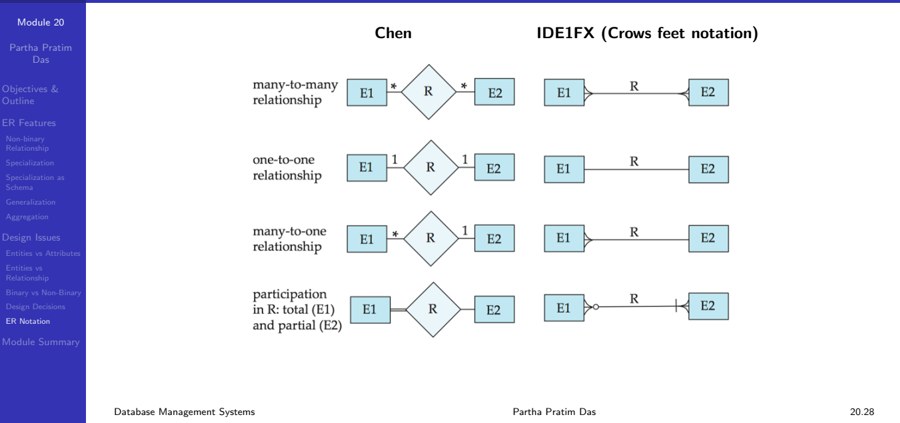
\includegraphics[height=0.8\textheight]{../Lecture 4.5_artifacts/image_000048_640192b192501ef84bdd5982d241c7ea6cf8f0a64ff3c41aa802cb5713b0de59.png}
    \end{center}
\end{frame}

\begin{frame}{Module Summary}
    \begin{block}{Summary}
        \begin{itemize}[<+->]
            \item Discussed the extended features of ER Model
            \item Deliberated on various design issues
        \end{itemize}
    \end{block}
    \vspace{2em}
    \begin{center}
    \small \textit{Slides used in this presentation are borrowed from \url{http://db-book.com/} with kind permission of the authors.} \\
    \small \textit{Edited and new slides are marked with 'PPD'.}
    \end{center}
\end{frame}

\end{document}
